\begin{figure}
  \centering
  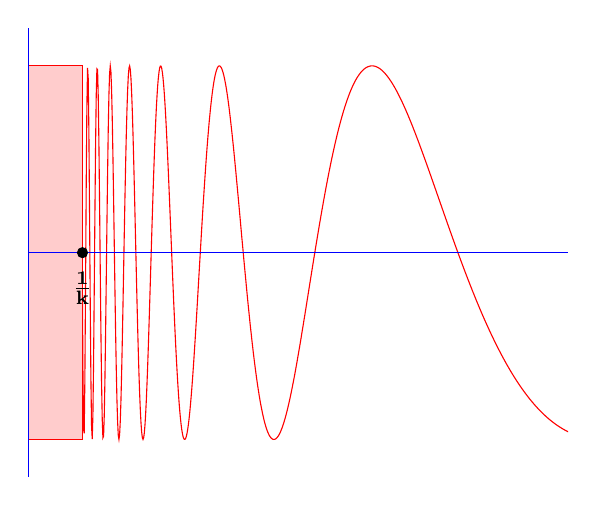
\begin{tikzpicture}
    \begin{axis}[axis lines=middle, xmin = 0 , ymin = -1.2 , ymax = 1.2 , xmax = 0.2, xtick=\empty, ytick=\empty, axis line style={color=blue, line width=0.6pt, -}, axis on top ]
      \addplot[domain=0.01:1, samples = 4000, color = red]{sin((deg(1/x)))};
      \addplot[draw=red, fill=red!20] coordinates {(0,-1) (0.02,-1) (0.02,1) (0,1)} \closedcycle ;
      \addplot[
  only marks,
  mark=*,
  mark size=1.8pt,
  color=black
] coordinates {(0.02,-0.00)};
\node[below] at (axis cs:0.02,-0.05) {$\mathbf{\frac1k}$};
    \end{axis}
  \end{tikzpicture}
\end{figure}
